\documentclass[a4paper, 10pt]{article}

\usepackage{INTERSPEECH2021}

\usepackage[linesnumbered,ruled,vlined]{algorithm2e}
\usepackage[hidelinks]{hyperref}
\usepackage{cleveref}
\usepackage{xcolor,soul,framed} %,caption
\usepackage{graphicx}
\usepackage{amsmath}
\usepackage{url}
\usepackage{cite}
\usepackage[super]{nth}
\usepackage[para]{threeparttable}
\usepackage{float}
\usepackage{tabularx}
\usepackage{amssymb}
\usepackage{amsfonts}
\usepackage{mathtools}
\usepackage{breakurl}

\newcommand*{\thead}[1]{%
\multicolumn{1}{c}{\bfseries\begin{tabular}{@{}c@{}}#1\end{tabular}}}

\def\UrlBreaks{\do\/\do-}

\DeclareMathOperator*{\argmax}{arg\,min}

\title{\LARGE{Subjectivity and Polarity Classification with Deep models}\\
\large{\textit{Final Project of the Natural Language Understanding Course}}}
\name{Matteo Guglielmi (232088)}

\address{University of Trento}
\email{matteo.guglielmi@studenti.unitn.it}

% CLI command to count words :  texcount -inc Final-Report.tex file wise
%                               texcount -inc -total Final-Report.tex   total words

\begin{document}

\maketitle

\begin{abstract}
    This work focuses on explaining the salient steps taken to implement a Sentiment Analysis algorithm that consists in \textit{Subjectivity} and \textit{Polarity Classification}.\\
    More in detail, a custom model is compared to a baseline in order to highlight the improvements achieved. To carry out this project, three different datasets were used : 
    the "\texttt{MovieReviews}" and  "\texttt{Subjectivity}" datasets both downloaded from the NLTK python module and the public "\texttt{IMDB}" dataset dowloaded from Kaggle\cite{kaggle}.\\
\end{abstract}


\textbf{\textit{Index Terms ---}} BertModel, BertTokenizer, BertForSequenceClassification, polarity classification, subjectivity detection, transformer,
pre-trained


% (approx. 100 words)

\vspace{-0.5cm}
\section{Introduction}
\label{sec:intro}
Sentiment analysis consists in performing sentence classification with the final goal to predict whether a sentence/review/comment expresses a positive or negative sentiment.
It is a very important task in the field of Natural Language Processing (NLP) and has been studied for many years being a very challenging task due to the 
presence of negation, sarcasm, irony, and other linguistic phenomena that make the job difficult.\\ 
%From a commercial point of view, sentiment analysis is a very important task since it can be used to automatically analyze the opinion of the customers about a product or 
%a service. For the latter reason, many industries are interested in this specific application to understand the degree of appreciation a specific product has.\\
In this work I'll be comparing two different models to perform sentiment and subjectivity classification. 

\vspace{-0.25cm}
\subsection{Baseline}
\label{subsec:basemodel}
The baseline model consists of:
\begin{itemize}
    \item a \texttt{CountVectorizer}\cite{vectorizer}, which acts as an encoder, to extract the features from the text;
    \item a \texttt{Na\"{i}ve Bayes}\cite{naive} classifier to perform the final classification.
\end{itemize}
It is worth mentioning that both datasets were pre-processed applying double negative marking (double negations corresponds to a neutral effect).
More in detail, the step-by-step procedure used to perform the classification is the following:
\begin{enumerate}
    \item Pre-processing: the text is pre-processed by collapsing the several sentences in documents and the double negations are marked;
    \item Feature extraction: text from the Subjectivity dataset is encoded using a \texttt{CountVectorizer};
    \item Classification: the encoded text from the previous point is classified using a \texttt{Na\"{i}ve Bayes} classifier;
    \item Evaluation: the classification is evaluated using a 10-fold cross-validation procedure exploiting the \texttt{accuracy} metric to address the overall performances;
    \item Filtering: the trained model is used to filter the objective sentences from the Movie Review dataset;    
    \item Feature extraction: the text belonging to the Movie Review dataset, after being processed as point (1), is encoded using a \texttt{CountVectorizer} as point (2);
    \item Classification: the encoded text is classified using a \texttt{Na\"{i}ve Bayes} classifier as point (3);
\end{enumerate}
\vspace{-0.25cm}
\subsection{Proposed model}
The proposed model follows the same logic of the baseline but with a completely different approach.
Very briefly, the proposed model consists in using :
\begin{itemize}
    \item a \texttt{Bert Tokenizer} \cite{tokenizer} to extract the features from the text and a \texttt{BertModel} \cite{model} to derive the embeddings;
    \item a small \texttt{BiLSTM} network used to filter objective movie reviews from the Movie Review dataset, accepting the output of the previous point as input;
    \item a \texttt{BertForSequenceClassification} to perform the final classification on the MovieReviews dataset as a whole.
\end{itemize}


% (approx. 200 words)

\section{Task formalization}
Sentiment analysis is the use of natural language processing and text analysis to identify, extract and quantify affective states and subjective information.\\
As previously mentioned, sentiment analysis is deployed in different fields to give voice to the customers and for the companies to receive a feedbacks through the analysis of forums or reviews.\\
With the raise of deep learning, it is possible to deal with very difficult scenarios, e.g. when the opinions are not explicitly expressed.\\
In the specific case of this assignment, the goal is to build a machine learning/deep learning model capable of performing subjectivity and polarity classification comparing the achieved results to a baseline model.\\
More precisely, the aforementioned model needs to perform:
\begin{itemize}
    \item sentiment classification : the automated process of identifying opinions in text and labeling them as positive, negative, or neutral, based on the emotions expressed within them. In this specific case, the Subjectivity dataset presentes only the positive and negative tag reducing the problem to a binary classification task;
    \item polarity classification which consists in labeling a text as subjective or objective.
\end{itemize}



% (approx. 200-500 words)

\vspace{-0.25cm}
\section{Data description and analysis}
\label{sec:data} 
\subsection{Movie reviews dataset}
\label{subsec:mr}
The movie reviews dataset used in this work is directly deployed by the \texttt{nltk.corpus} python package whose characteristics are the following :
\begin{itemize}
    \item number of words : \numprint{1583820};
    \item lexicon size : \numprint{39768};
    \item categories : 'neg', 'pos'.
\end{itemize}
Each movie review has a file id associated with it used for its identification containing all the relative information.
%The dataset presents itself in a peculiar structure. As mentioned to each review corresponds a file containing the relative information, all files are then added to a list, 
%each with an associated label.\\
This dataset is used just for evaluation, since the amount of reviews is too small to perform a proper fine-tuning operation of the BertForSequenceClassification (see 
\textbf{\Cref{subsec:custom}}).
%For this reason, the whole dataset has been used just to address the final polarity classifiaction accuracy.

\subsection{Subjectivity dataset}
\label{subsec:subj}
The subjectivity dataset is provided by the \texttt{nltk.corpus} python module as well.\\ 
The main characteristics of this dataset are :
\begin{itemize}
    \item vocabulary size : \numprint{240576};
    \item lexicon size : \numprint{23906};
    \item classes : 'obj', 'subj';
    \item total number of sentences : \numprint{10000}.
\end{itemize}
In this specific case, there are just two unique file ids corresponding to the documents containing the objective and subjective sentences. 
%The datastructure used in the code consists of the union of those two files.

\subsection{IMDB dataset}
\label{subsec:imdb}
The IMDB Dataset has \numprint{50000} movie reviews for natural language processing or text analytics ~\cite{kaggle}. This dataset can be used for binary sentiment 
classfication and it provides \numprint{25000} highly polar samples for training and \numprint{25000} samples for testing. More information reguarding this dataset can 
be found at ~\cite{refe}.

% (approx. 200-500 words)

\section{Model}
\label{sec:model}
For the proposed task, I have decided to use a simple \texttt{Na\"{i}ve Bayes classifier} as baseline, following the logical procedure explained in the \nth{11} laboratory 
~\cite{lab11}.\\
Once the baseline performances were addressed, I tried to devise a completely different procedure by making use of more complex deep architectures. \\

\vspace{-1.5em}
\subsection{Architectures}
Baseline and custom model follow the same logical flow leading to both subjectivity and polarity classification, although the single components are complitely different.
%In particular, the baseline approach (\textbf{\Cref{subsec:baseline}}) consists in a pure shallow machine learning procedure; 
%whereas, for the custom model, I decided to opt for a deep architecture-based techinque.\\
The logical salient steps taken in both cases are :
\begin{enumerate}
    \item extract the encodings of each sentence leading to a vector representation;
    \item train a ML/DL model upon the \texttt{subjectivity dataset} and save the weights;
    \item use the pre-trained model from the previous point to filter out the objective sentences;
    \item perform polarity classification upon the sentences predicted as subjective and address the performances through the \texttt{accuracy} metric.
\end{enumerate}

\subsection{Na\"{i}ve Bayes classifier baseline}
\label{subsec:baseline}
Concerning the baseline, the followed workflow is well expressed by \texttt{Algorithm \ref{alg:baseline}}:
\begin{algorithm}
    \SetAlgoLined
    \DontPrintSemicolon
    \KwIn{subj\_dt, mr\_dt}    
    \KwOut{subj\_acc, pol\_acc}
    \CommentSty{\color{blue}}
        \tcc{
            subj\_dt: list of (sentences,label)\; 
            mr\_dt: list of (sentences,label),\; 
            subj\_acc: subjectivity accuracy,\;
            pol\_acc: polarity accuracy
        }
        subj\_features $\gets$ FitVectorizerOn(subj\_dt)\;
        subj\_scores $\gets$ 10-fold-cross-val(NB\_clf, subj\_features, subj\_labels)\;
        \tcc{ 
            considering best estimator
        }
        best\_clf $\gets$ $\underset{\text{clf}}{\mathrm{argmax}} \bigr($subj\_scores$\bigl)$\;
        subj\_sents $\gets$ filter\_objectivness(best\_clf(pol\_dt))\;
        \tcc{ new vectorizer and clf }
        pol\_features $\gets$ FitNewVectorizerOn(subj\_sents)\;
        pol\_scores $\gets$ 10-fold-cross-val(New\_NB\_clf, pol\_features, pol\_labels)\;
    \caption{Steps performed in baseline model.}
    \label{alg:baseline}
\end{algorithm}

\vspace{-2.0em}
\subsection{Custom model}
\label{subsec:custom}
On the other side, my proposed implementation adopts only deep models to carry out this assignment. In particular:
\begin{itemize}

    \item the \texttt{CountVectorizer} used as embedder in the baseline has been substituted with a small pipeline composed of:
        \begin{itemize}

            \item a pre-trained BertTokenizer ~\cite{tokenizer} based on WordPiece ~\cite{wordpiece} used to break text into tokens, 
                pad sentences to a maximum of  $512$ letters allowed by BERT, truncate to \texttt{max\_length} longer phrases 
                and convert text into float tensors;

            \item a pre-trained BertModel ~\cite{model} to extract text encondings to be used later on in the pipeline. These encodings
                are obtained by extracting the output of the transformer last hidden state as done in ~\cite{mtl}.

        \end{itemize}

    \item the Na\"{i}ve Bayes classifier has been changed with: 
        \begin{itemize}

            \item a simple \texttt{BiLSTM} network consisting of : 
                \begin{enumerate}

                    \item a \texttt{BiLSTM} layer which accepts an output with a $768$ long feature vector (output of the last hidden 
                        layer of BertModel) with an hidden dimension of $128$;

                    \item a \texttt{Dense} layer with an output size of $64$ and a ReLU activation function to flatten the feature maps;

                    \item a \texttt{Dropout} layer to reduce at the minimum possible the computational load with a probability of $0.35$;

                    \item and finally a \texttt{Linear} layer to produce a binary out.

                \end{enumerate}
                to perform subjectivity classification;

            \item a \texttt{BertForSequenceClassification} ~\cite{sequence} model fine-tuned for one epoch 
                (to shorten training time) (results in \textbf{\Cref{fig:singleepoch}}) upon the IMDB Dataset (\textbf{\Cref{subsec:imdb}}) for performing polarity classification 
                upon the \texttt{MovieReviews} dataset (\textbf{\Cref{subsec:mr}}).

        \end{itemize}
\end{itemize}

\subsection{Optimizers}
\label{subsec:opt}
In this work, two different optimizers have been used:
\begin{enumerate}
    \item \texttt{Adam} optimizer has been used to update the BiLSTM model parameters. It's been chosen among the other options due to
        its ability to converge quickly;
    \item \texttt{AdamW} optimizer has been used to train the BertForSequenceClassification model. This particular variant of the classic 
        Adam optimizer has been used because it's the default training option when using the \texttt{Trainer()} interface ~\cite{trainer} 
\end{enumerate}

\subsection{Experiments}
\label{subsec:exp}
Several experiments were run using the proposed model (\textbf{\Cref{subsec:custom}}). In particular, I initially tried to use the output 
of the pre-trained BertModel instance to predict the polarity scores after filtering out the objective sentences. \\
In this case the issue was that this model ~\cite{model} outputs by definition $5$ possible labels, ranging from $0 \to 5$. As a consequence,
I tried mapping the two lowest scores ($0,1$) to the 'negative' label and the upper scores ($4,5$) to the 'positive' one, leaving  score
$3$ as an indicator of uncertainty and misclassification. After analysing the predictions, the model turned out as heavily 
undecided, predicting mostly $3$.\\
With these results as a reference, I tried to "flat" the $5$ predicted labels to a binary score appending a linear layer with a Sigmoid activation function
in combination with a \texttt{BCELoss()} ~\cite{bce}. \\
After some research, I found out that a "C-class version" for the canonical BertModel already existed (\texttt{BertForSequenceClassification}).\\
Thanks to that, I was able to exploit a pre-trained very deep model to perform binary ($C=2$) text classification combined with a binary cross-entropy
loss used during the fine tuning procedure (it is worth mentioning that the Trainer class is responsible for computing some sort of loss 
and returning it as output if no \texttt{compute\_loss()} method is specified, as discussed in ~\cite{stack}). \\
Further experiments were conduced attempting to reduce the amount of encoded tokens in the MovieReviews dataset by clearing the source text from  elements such as stopwords, 
numbers, HTML special entities, hyperlinks, hashtags, punctuation (besides exclamation marks), words with less than $2$ letters, usernames (@USERNAME) and tickers. 
It turned out that both the BiLSTM model and the BertForSequenceClassification achieved better results without filtering (see \textbf{\Cref{tab:filter}}), proving these 
elements as relevant to the context.
\begin{center}
        \vspace{-3.0em}
        \begin{table}
            \let\TPToverlap=\TPTrlap    
            \centering
            \caption{Effects of filtering upon polarity dataset.}
            \vspace{-1.0em}
            \begin{threeparttable}
                    \begin{tabular}{cc}
                        \toprule
                        \textbf{Custom Model} & \textbf{Accuracy} \\ \hline
                        Without filtering & 0.9283 \\
                        With filtering & 0.8642 \\
                        \bottomrule
                    \end{tabular}
                    \label{tab:filter}
            \end{threeparttable}
        \end{table}
\end{center}

% (approx. 500-800 words)

\section{Evaluation}
\label{sec:eval}
The purpose of this section is to explain and show the obtained results across different runs. In particular, it is worth mentioning that
lots of default valued hyper-parameters have been used such as:
\begin{itemize}
    \item \textit{batch size}, for both the training of the BiSTM (\Cref{subsec:subj}) and the final polarity evaluation procedure, of $128$
        samples. In the case of the binary classifier (~\cite{sequence}), a batch size of $64$ has been used;
    \item concerning the \textit{dataset split} dimensions:
        \begin{itemize}
            \item the subjectivity dataset into training set ($80\%$) and test set ($20\%$). The training set has been further splitted 
            considering a randomly sampled $10\%$ for evaluation pruposes;
            \item the IMDB dataset has been splitted following the built-in splitting format of the dataset itself ($25K$ samples for training
            and $25K$ sampels for evaluation)
        \end{itemize}
    \item during the training procedure an \textit{early stopper} has been used to implement an early stopping techinque. To do so, the 
        difference between the accuracy at the previous run and the current one is investiagate. If the latter is grater than $MIN\_DELTA=0.075$, 
        then the training procedure is interrupted and the last model saved;
    \item the BiLSTM model has been trained for $10$ \textit{epochs} and the binary classifier just for one (for time reasons);
    \item regarding the BiLSTM model, the multiple runs have been performed using a randomly selected seeds: $[91, 11, 57, 822, 19]$;
    \item for the AdamW and Adam optimiers, the learning rates used are $0.001$ and $0.0002$ respectively. 
\end{itemize}


\subsection{Evaluation metric}
\label{subsec:metric}
Across the different models, several evaluation metrics have been used. 
\subsubsection{Baseline}
Concerning the baseline, a simple \texttt{accuracy} metric has been used across a 10-fold cross validation procedure.
\subsubsection{Custom model}
As regards my proposed model, different evaluation metrics have been used for the different components:
\begin{itemize}
    \item for the BiLSTM model, as well as for the final evaluation on the polarity dataset, to detect subjectivity labels, a simple cumulative accuracy metric, defined as the sum of all the agreeements
    across all the batches over the number of samples in the training set, has been used;
    \item for the \textit{BertForSequenceClassification} instance an ensamble of metrics has been computed, exploiting the 
    \texttt{accuracy\_score} and \texttt{precision\_recall\_fscore\_support} methods provided by the \texttt{sklearn} python module. 
    In particular, the function used to compute these metrics can be analysed in \textbf{\Cref{alg:binaryclf}}
    \item as for the BiLSTM model, also for the final polarity classification step a cumulative accuracy has been used, where the agreeements
    between the predictions given by the pre-fine-tuned binary classifier and the ground truth are investigated and quantified.
\end{itemize}


\begin{algorithm}
    \SetAlgoLined
    \DontPrintSemicolon
    \KwIn{pred}    
    \KwOut{accuracy, f1, precision, recall}
    \CommentSty{\color{blue}}
    precision, recall, f1, \_  $\gets$ precision\_recall\_fscore\_support(labels, preds, average='binary')\;
    acc $\gets$ accuracy\_score(labels, preds)\;

    return\{\;
            \hspace{5mm}'accuracy': acc,\;
            \hspace{5mm}'f1': f1,\;
            \hspace{5mm}'precision': precision,\;
            \hspace{5mm}'recall': recall\;
        \}

\caption{Metric computation function for Trainer interface.}
\label{alg:binaryclf}

\end{algorithm}

Of course, the overall objective is to maximise the accuracy on both subjectivity and polarity datasets by minimizing the losses used during 
the training procedure as application of the maximisation of the posterior probabilities.

\subsection{Results}
\label{subsec:res}
In this particular section, the results obtained across different runs and experiments are analysised as much in detail as possible.\\
\begin{figure}
    \centering
    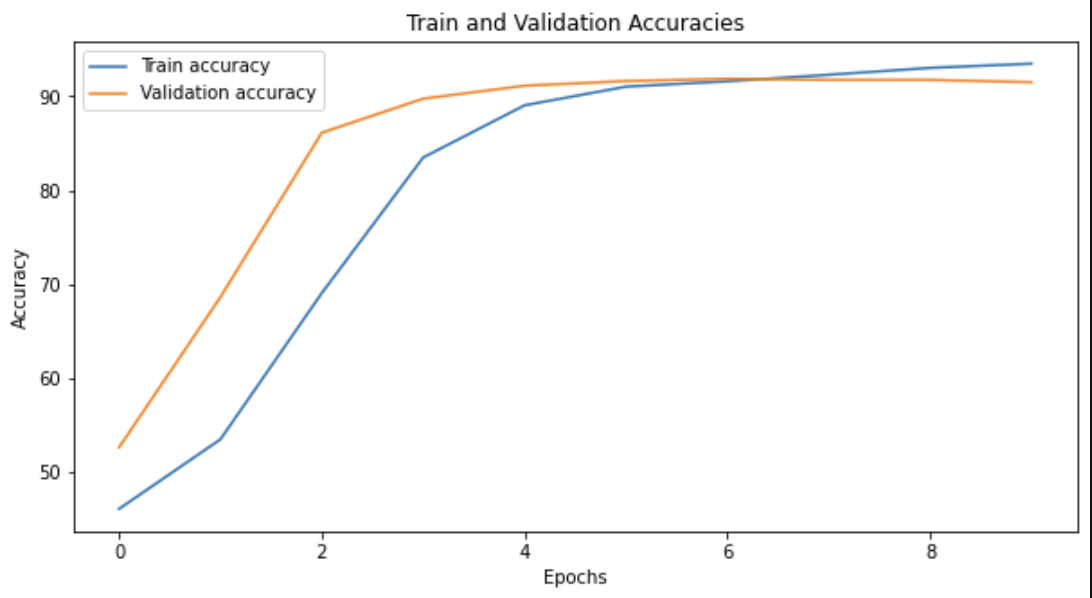
\includegraphics[scale=0.28]{Images/singlerunacc.png}
    \vspace{-1.0em}
    \caption{BiLSTM model training and evaluation accuracies on a single run.}
    \vspace{-1.0em}
    \label{fig:singlerunacc}
\end{figure}

\begin{figure}
    \centering
    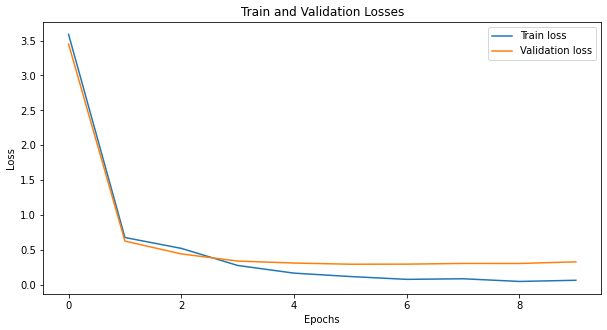
\includegraphics[scale=0.28]{Images/singlerunloss.png}
    \vspace{-1.0em}
    \caption{BiLSTM model training and evaluation losses on a single run.}
    \vspace{-1.0em}
    \label{fig:singlerunloss}
\end{figure}


In \textbf{\Cref{fig:singlerunacc}} and \textbf{\Cref{fig:singlerunloss}} it is possible to respectively appreciate the training and 
evaluation accuracies and losses, on a single run for the BiLSTM model (discussed in \Cref{subsec:cutsom}). \\
Since a single run is not very expressive and fully reliable, I decided to perform a 5-fold cross validation addressing both the average 
accuracy as well as the variance across the different runs (for details refer to \Cref{tab:crossval}).\\

\begin{center}
    \begin{threeparttable}
    \caption{5-fold cross validation subjectivity results using BiLSTM model}
        \begin{tabular}{cc}
            \toprule
            \thead{Seeds} & \thead{Accuracy} \\
            \hline
            $91$ & $89.5$ \\
            $11$ & $90.8$ \\
            $57$ & $91.05$\\
            $822$ & $90.25$\\
            $19$ & $89.1$ \\
            \hline
            Avg. Acc. & $90.14$ \\
            \hline
            Acc. Var. & $0.74$ \\
            \bottomrule
        \end{tabular}
        \label{tab:crossval}
    \end{threeparttable}
\end{center}

The main reason behind using a BiLSTM model is to try to better catch the dependencies between the words in a sentence. The results turned out to be worse than the ones obtained with the baseline from 
the cumulative accuracy perspective but better in terms of consistency and stableness. Indeed, using the same evaluation metric, the average statistics, listed in \Cref{tab:comparison}, 
shows that the baseline reaches a better percentual average accuracy but a higher variance across the different runs, i.e. seems to be more unstable and inconsistent.\\

\begin{center}
    \begin{threeparttable}
    \caption{Comparison between the baseline and the BiLSTM model}
        \begin{tabular}{ccc}
            \toprule
            \thead{Model} & \thead{Accuracy} & \thead{Variance}\\
            \hline
            Baseline & $90.75\%$ & $0.00013765$ \\
            Custom Model & $90.14\%$ & $5.534000000000004e-05$\\
            \bottomrule
        \end{tabular}
        \label{tab:comparison}
    \end{threeparttable}
\end{center}

Investigating the final results on the polarity dataset, it is possible to appreciate that the proposed model reaches a better accuracy than the baseline, as shown in \Cref{tab:finalres}.\\
It is worth mentioning that the "x" on the \texttt{accuracy} column of the table means that the model has not been tested multiple times on the polarity dataset since the latter is used just for evaluation
purposes as discussed in \Cref{subsec:mr}.\\


\begin{center}
    \begin{threeparttable}
    \caption{Comparison between the baseline and the proposed model}
        \begin{tabular}{ccc}
            \toprule
            \thead{Model} & \thead{Accuracy} & \thead{Variance}\\
            \hline
            Baseline & $83.2\%$ & $0.00112$\\
            Custom Model & $92.83\%$ & x\\
            \bottomrule
        \end{tabular}
        \label{tab:finalres}
    \end{threeparttable}
\end{center}


\vspace{-.5cm}
\section{Conclusion}
\label{sec:end}
To summarise, in this work I've presented an alternative method for performing subjectiviy detection and polarity classification explaining the most salient steps taken to 
carry out this task as well as possible limitations and improvements.\\
As pointed out during the report, the baseline model used for this task is a simple shallow model, which is in most of the cases not the best choice for such complex problems. 
In response to this I also tested a deep learning model able to perform the task with a better accuracy (\textbf{\Cref{subsec:res}}).\\
As final remarks, I would like to point out that the results obtained in this work are not intended as optimal, but they are a good starting point for further improvements. 
In particular, for future improvements I would focus on dealing with the limitation of using the Bert model as encoder trying to use other variants that are not limited to 
a maximum sequence length. 




\bibliographystyle{IEEEtran}
\bibliography{mybib.bib}

\end{document}
